\documentclass[../main]{subfiles}
\begin{document}
    \section{Gravedad Linealizada}

La expresión a primer orden sobre una métrica plana se escribe como:
\begin{equation}
    g_{\mu\nu}=\eta_{\mu\nu}+h_{\mu\nu} \quad \text{con} \quad ||h_{\mu\nu}|| << 1,
\end{equation}
donde $h_{\mu\nu}$ es la perturbación sobre $\eta_{\mu\nu}$, la inversa de $g_{\mu\nu}$, viene dada por:
\begin{equation}
    \begin{split}
        g^{\mu\nu}&=\eta^{\mu\nu}-h^{\mu\nu} \\
        g^{\mu\alpha}g_{\mu\beta}&=(\eta^{\mu\alpha}-h^{\mu\alpha})(\eta_{\mu\beta}+h_{\mu\beta}) \\
        \delta^{\alpha}_{\beta}&=\delta^{\alpha}_{\beta}+\eta^{\mu\alpha} h_{\mu\beta}-h^{\mu\alpha}\eta_{\mu\beta}+\mathcal{O}(h^2)\\
        \eta^{\mu\alpha}h_{\mu\beta} &\cong h^{\mu\alpha}\eta_{\mu\beta}
    \end{split}
\end{equation}
vemos que $\eta^{\mu\alpha}$ mapea las componentes covariantes de $h_{\mu\beta}$ en sus componentes contravariantes a primer orden en $h$ 
\begin{equation}
    h^{\alpha}_{\beta} \cong h^{\alpha}_{\beta}=h^{\alpha}_{\beta}
\end{equation}
por lo que la métrica $\eta_{\mu\nu}$ puede ser usada para subir los índices de la perturbación $h_{\mu\nu}$.

Los símbolos de Christoffel vienen dados por:
\begin{equation}
    \Gamma^{\alpha}_{\beta\gamma}=\dfrac{1}{2}\eta^{\alpha\lambda}(\partial_{\beta}h_{\lambda\gamma}+\partial_{\gamma}h_{\beta\lambda}-\partial_{\lambda}h_{\beta\gamma}),
\end{equation}
y el tensor de Riemann a primer orden en $h$:
\begin{equation}
    \begin{split}
        R^{\sigma}_{\mu\rho\nu}&=\partial_{\rho} \Gamma^{\sigma}_{\mu\nu}-\partial_{\nu}\Gamma^{\sigma}_{\mu\rho}+\underbrace{\Gamma^{\lambda}_{\mu\nu}\Gamma^{\sigma}_{\rho\lambda}-\Gamma^{\lambda}_{\rho\mu}\Gamma^{\sigma}_{\nu\lambda}}_{\mathcal{O}(h^2)} \\
        &=\dfrac{1}{2}\eta^{\sigma\lambda}(\partial_{\rho}\partial_{\mu}h_{\nu\lambda}-\partial_{\rho}\partial_{\lambda}h_{\mu\nu}-\partial_{\nu}\partial_{\mu}h_{\rho\lambda}+\partial_{\nu}\partial_{\lambda}h_{\mu\rho})
    \end{split}
\end{equation}
donde el tensor de Ricci y el escalar de Ricci:
\begin{align}
    R_{\mu\nu}&=\dfrac{1}{2}(\partial^{\lambda}\partial_{\mu}h_{\nu\lambda}-\Box h_{\mu\nu}+\partial^{\lambda}\partial_{\nu}h_{\mu\lambda}-\partial_{\mu}\partial_{\nu}h^{\lambda}_{\lambda})\\
    R&=\partial^{\mu}\partial^{\nu}h_{\mu\nu}-\Box h^{\lambda}_{\lambda}
\end{align}

Las ecuaciones de Einstein se reducen:
\begin{equation}
    \dfrac{1}{2}\left\{\partial^{\lambda}\partial_{\mu}h_{\nu\lambda}+\partial^{\lambda}\partial_{\nu}h_{\mu\lambda}-\Box h_{\mu\nu}-\partial_{\mu}\partial_{\nu}h-(\partial^{\rho}\partial^{\sigma}h_{\rho\sigma}+\Box h^{\lambda}_{\lambda})\eta_{\mu\nu}\right\}=8\pi G T_{\mu\nu}(\vec{x}, t)
\end{equation}
para uan fuente de energía dada por $T_{\mu\nu}$ que varía con $t$.

\subsection{Simetría Gauge o de calibre}

Bajo transformaciones infinitesimales $x^{\mu} \rightarrow x^{\mu}+\xi^{\mu}$, la métrica $g_{\mu\nu}$ cambia por:
\begin{equation}
    \begin{split}
        \delta g_{\mu\nu}&=\nabla_{\mu} \xi_{\nu}+\nabla_{\nu}\xi_{\mu} \\
        \delta(\eta_{\mu\nu}+h_{\mu\nu})&=(\partial_{\mu}\xi_{\nu}+\partial_{\nu}\xi_{\mu}-\underbrace{\Gamma^{\alpha}_{\mu\nu}\xi_{\alpha}}_{\mathcal{O}(h\xi)}-\underbrace{\Gamma^{\alpha}_{\nu\mu}\xi_{\alpha}}_{\mathcal{O}(h\xi)}) \\
        \delta h_{\mu\nu}&=\partial_{\mu} \xi_{\nu}+\partial_{\nu} \xi_{\mu}
    \end{split}
\end{equation}

Luego:
\begin{equation}
    h_{\mu\nu} \ \rightarrow \ h_{\mu\nu}+\partial_{\mu}\xi_{\nu}+\partial_{\nu}\xi_{\mu}.
\end{equation}

Entonces, en analogía con el electromagnetismo, se puede imponer un gauge para fijar las componentes de $h_{\mu\nu}$. 

Usando el gauge de \textcolor{red}{de Donder}:
\begin{equation}
    \begin{split}
        g^{\mu\nu}\Gamma^{\sigma}_{\mu\nu}&=0\\
        \eta^{\mu\nu}\left\{\dfrac{1}{2}\eta^{\sigma\rho}(\partial_{\mu}h_{\rho\nu}+\partial_{\nu}h_{\rho\mu}-\partial_{\rho}h_{\mu\nu})\right\}&=0\\
        \partial^{\nu}h^{\sigma}_{\nu}+\partial^{\mu}h^{\sigma}_{\mu}-\partial^{\sigma}h^{\lambda}_{\lambda}&=0\\
        \partial^{\nu}h_{\nu\sigma}-\dfrac{1}{2}\partial_{\sigma}h&=0
    \end{split}
\end{equation}

Las ecuaciones de Einstein en este gauge se reducen a:
\begin{equation}
    \Box h_{\mu\nu}-\dfrac{1}{2}\Box h \eta_{\mu\nu}=-16\pi G T_{\mu\nu},
\end{equation}
definiendo 
\begin{equation}
    \begin{split}
        \bar{h}_{\mu\nu}&=h_{\mu\nu}-\dfrac{1}{2}h \eta_{\mu\nu} \\
        \Box \bar{h}_{\mu\nu}&=-16\pi G T_{\mu\nu}
    \end{split}
\end{equation}

Reduciendose a una ecuación de onda.

\subsection{Límite Newtoniano}

En este límite $h_{\mu\nu}(\vec{x}, t)=h(\vec{x})$:
\begin{equation}
    \begin{split}
        \Box \bar{h}_{\mu\nu}&=-16\pi G T_{\mu\nu} \\
        \vec{\nabla} \bar{h}_{\mu\nu}&=-16\pi G T_{\mu\nu}
    \end{split}
\end{equation}

Escogiendo: $\bar{h}_{00}=-4\Phi(\vec{x})$ y $\bar{h}_{0i}=h_{ij}=0$
\begin{equation}
    \begin{split}
        -4\vec{\nabla}^2 \Phi (\vec{x})&=-16\pi G\rho \\
        \vec{\nabla}^2 \Phi(\vec{x})&=4\pi G\rho
    \end{split}
\end{equation}
que es la ecuación de Poisson.

El elemento de línea en este límite:
\begin{equation}
    \mathrm{d}s^2=-(1+2\Phi(\vec{x}))\mathrm{d}t^2+(1-2\Phi(\vec{x}))\mathrm{d}\vec{x}^2
\end{equation}
coincide con el caso de gravedad Newtoniana.

\section{Soluciones a la ecuación de onda}

Para la ecuación en el vacío:
\begin{equation}
    \Box \bar{h}_{\mu\nu}=0
\end{equation}
tiene soluciones:
\begin{equation}
    \bar{h}_{\mu\nu}=\Re(A_{\mu\nu}e^{ik_{\mu}x^{\mu}})
\end{equation}
de donde $k_{\mu}$ debe ser un vector nulo que cumple con:
\begin{equation}
    k_{\mu}k^{\mu}=0
\end{equation}
donde $k^{\mu}=(\omega, \vec{k})$ con $\omega$ como la frecuencia de las ondas gravitacionales 
\begin{equation}
    \omega=\pm |\vec{k}| \quad \text{y} \quad \dv{\omega}{|\vec{k}|}=1,
\end{equation}
por lo que las ondas gravitacionales viajan a la velocidad de la luz.

La matriz $H_{\mu\nu}$, define la amplitud de la onda gravitacional con 10 componentes reducibles a 2 componentes independientes que definen la \textcolor{red}{polarización} de las ondas gravitacionales.

En el gauge de \textcolor{red}{de Donder}, la condición $\partial^{\mu}\bar{h}_{\mu\nu}=0$ implica que:
\begin{equation}
    k^{\mu}A_{\mu\nu}=0,
\end{equation}
definiendo la polarización como transversal a la dirección de propagación, estas ecuaciones definen 4 vínculos sobre $A_{\mu\nu}$. Sin embargo $A_{\mu\nu}$ satisface 
\begin{equation}
    \bar{h}_{\mu\nu} \ \rightarrow \ \bar{h}_{\mu\nu}+\partial_{\mu}\xi_{\nu}+\partial_{\nu}\xi_{\mu},
\end{equation}
para $\partial^{\mu}h_{\mu\nu}=0$, $\xi_{\mu}$ satisface:
\begin{equation}
    \Box \xi_{\mu}=0, \ \xi_{\mu}=x_{\mu}e^{i\tilde{k}_{\mu} x^{\mu}}
\end{equation}
entonces para $\bar{h}_{\mu\nu}=A_{\mu\nu}e^{ik_{\mu}x^{\mu}}$ en el plano transverso:
\begin{equation}
    A_{\mu\nu} \ \rightarrow \ A_{\mu\nu}+i(\tilde{k}_{\mu}x_{\nu}+\tilde{k}_{\nu}x_{\mu}-\tilde{k}^{\sigma}x_{\sigma}\eta_{\mu\nu}),
\end{equation}
por lo que podemos escoger $A_{0\mu}=0$ y $A^{\mu}_{\mu}=0$ como soluciones que dejan $A_{\mu\nu}$ invariante, entonces estas condiciones definen el gauge \textcolor{red}{transverso y sin traza}.

Las soluciones para $\bar{h}_{\mu\nu}$ en este gauge en la dirección $\hat{z}$ se escriben como:
\begin{equation}
    \bar{h}^{\Pi}_{\mu\nu}(t, z)=
    \begin{pmatrix}
        0 & 0 & 0 & 0 \\
        0 & \textcolor{red}{h_+} & \textcolor{blue}{h_{\times}} & 0 \\
        0 & \textcolor{blue}{h_\times}& \textcolor{red}{-h_+} &  0\\
        0 & 0 & 0 & 0
    \end{pmatrix}
    \cos[\omega(t-z)]
\end{equation}
escrito en términos del elemento de línea $\mathrm{d}s^2$
\begin{equation}
    \begin{split}
        \mathrm{d}s^2&=-\mathrm{d}t^2+\mathrm{d}z^2+\left[1+h+\cos(\omega t-\omega z)\right]\mathrm{d}x^2+\left[1+h+\cos(\omega(t-z))\right]\mathrm{d}y^2\\
        &\quad +2h_x\cos(\omega(t-z))\mathrm{d}x\mathrm{d}y 
    \end{split}
\end{equation}

En general, podemos introducir el proyector $\Lambda_{ijkl}$ de la forma 
\begin{equation}
    \Lambda_{ijkl}(\hat{n})=P_{ik}P_{jl}-\dfrac{1}{2}P_{ij}P_{kl}
\end{equation}
donde $P_{il}$ viene dado por:
\begin{equation}
    P_{il}=\delta_{il}-n_i n_l
\end{equation}

Este proyector permite encontrar $\bar{h}^{\Pi}_{ij}$ en el gauge Transverso sin traza dado una solución de onda plana $h_{\mu\nu}$ en el gauge de de Donder:
\begin{equation}
    h^{\Pi}_{ij}=\Lambda_{ijkl}h_{kl}
\end{equation}

$\Lambda_{ijkl}$ satisface las siguientes propiedades:
\begin{enumerate}
    \item $\Lambda_{ijkl}\Lambda_{klmn}=\Lambda_{ijmn}$.
    \item $n^{i}\Lambda_{ijkl}=0$; $n^{j}\Lambda_{ijkl}=0$.
    \item $\Lambda_{iikl}=0$; $\Lambda_{ijkk}=0$.
\end{enumerate}

Para estudiar el efecto de una onda gravitacional sobre varias parrticulas usamos la ecuación de la desviación geodésica:
\begin{equation}
    \dfrac{\mathrm{D}^2 B^{\mu}}{\mathrm{D}\tau^2}=-R^{\mu}_{\nu\rho\sigma}U^{\nu}U^{\sigma}B^{\rho} \quad \text{con} \quad \dfrac{\mathrm{D}}{\mathrm{D}\tau}=T^{\alpha}\nabla_{\alpha}
\end{equation}
donde $B^{\mu}$ es el vector de separación entre geodésicas vecinas. A primer orden en $h$, podemos aproximar la $U^{\mu}$ como 
\begin{equation}
    U^{\mu} \cong (1, 0, 0, 0)
\end{equation}
y el tiempo propio:
\begin{equation}
    \mathrm{d}\tau\approx \mathrm{d}t \quad \rightarrow \quad \dv{^2 B^{\mu}}{t^2}=-R^{\mu}_{0\rho 0}B^{\rho}
\end{equation}
luego usando la condición $h_{\mu 0}=0$, las componentes no nulas del tensor de Riemann vienen dadas por:
\begin{equation}
    R^{\mu}_{0\rho 0}=-\dfrac{1}{2}\partial^2_0 h^{\mu}_{\rho}
\end{equation}

La ecuación de la desviación geodésicas para $B^{\mu}$ satisface a primer orden en $h_{\mu\nu}$ 
\begin{equation}
    \dv{^2 B^{\mu}}{t^2}=\dfrac{1}{2}\dv{h^{\mu}_{\rho}}{t^2}B_{\rho}
\end{equation}
en el plano $z=0$ y para $h_{\mu\rho}=A^+_{\mu\rho}e^{i\omega t}$ 
\begin{equation}
    \begin{split}
        \dv{^2 B^1}{t^2}&=-\dfrac{\omega^2}{2}h_+ e^{i \omega t}B^1 \\ 
        \dv{^2 B^2}{t^2}&=+\dfrac{\omega^2}{2}h_+ e^{i \omega t}B^2
    \end{split}
\end{equation}

Que tiene soluciones para $A_+ << 1$(primer orden en $h$) donde hemos usado la forma matricial de $h_{\mu\nu}$, despues de fijar calibre. Estas ecuaciones tienen las siguientes soluciones:
\begin{equation}
    \begin{split}
        B^1(t)&=B^1(0)\left(1+\dfrac{1}{2}h_+ e^{i\omega t}+\mathcal{O}(h^2)\right)\\
        B^2(t)&=B^2(0)\left(1+\dfrac{1}{2}h_+ e^{i\omega t}+\mathcal{O}(h^2)\right)
    \end{split}
\end{equation}

Para $t=0$ sí las geodésicas con separación $B^{\mu}$ satisfacen sí en $t=0$ corresponde a un círculo:
\begin{equation}
    (B^1(0))^2+(B^2(0))^2=R^2,
\end{equation}
entonces como $B^1$ y $B^2$ son separables en la ecuación de la desviación geodésica, el modo $h_+$ corresponde a oscilaciones en estas geodésicas de la forma:

\begin{figure}[h]
    \centering
    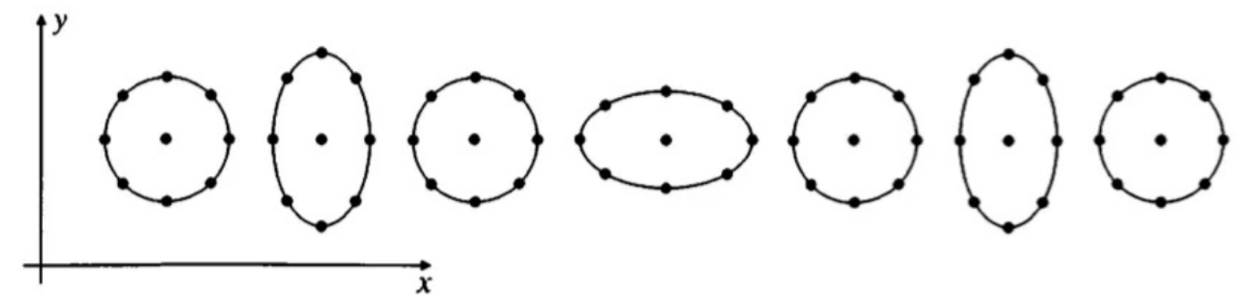
\includegraphics[width=.8\textwidth]{img/imgRG8.1.PNG}
    \label{fig8.1}
    \caption{Oscilación para $h_x$ al pasar una onda gravitacional. (Sean Carroll)}
\end{figure}

Adicionalmente, como en electromagnetismo, es posible definir \textcolor{red}{polarización circular} \textcolor{blue}{derecha} o \textcolor{blue}{izquierda} usando 
\begin{align}
    h_R&=\dfrac{1}{\sqrt{2}}(h_+ +ih_x)\\
    h_L&=\dfrac{1}{\sqrt{2}}(h_+ -ih_x)
\end{align}

\section{Producción de Ondas Gravitacionales}

Para estudiar la producción de ondas gravitacionales consideramos la ecuación no-homogénea de $h_{\mu\nu}$ 
\begin{equation}
    \Box \bar{h}_{\mu\nu}=-16\pi G T_{\mu\nu}
\end{equation}
donde $\bar{h}_{\mu\nu}$ es definido como:
\begin{equation}
    \bar{h}_{\mu\nu}=h_{\mu\nu}-\dfrac{1}{2}\eta_{\mu\nu}h
\end{equation}

Para una fuente de materia moviéndose a velocidades no-relativistas, la solución a la ecuación para $\bar{h}_{\mu\nu}$ viene dada por:
\begin{equation}
    \bar{h}_{\mu\nu}(t, \vec{x})=4G\int_{\Sigma}\mathrm{d}^3 y \dfrac{T_{\mu\nu}(t_r, y)}{|x-y|},
\end{equation}
donde $\Sigma$ es la región donde $T_{\mu\nu}$ está definido, $t_r$ es el tiempo retardado al encontrar la función de Green para el problema homogéneo y se define como:
\begin{equation}
    t_r=t-|\vec{x}-\vec{y}|
\end{equation}
\begin{figure}[h]
    \centering
    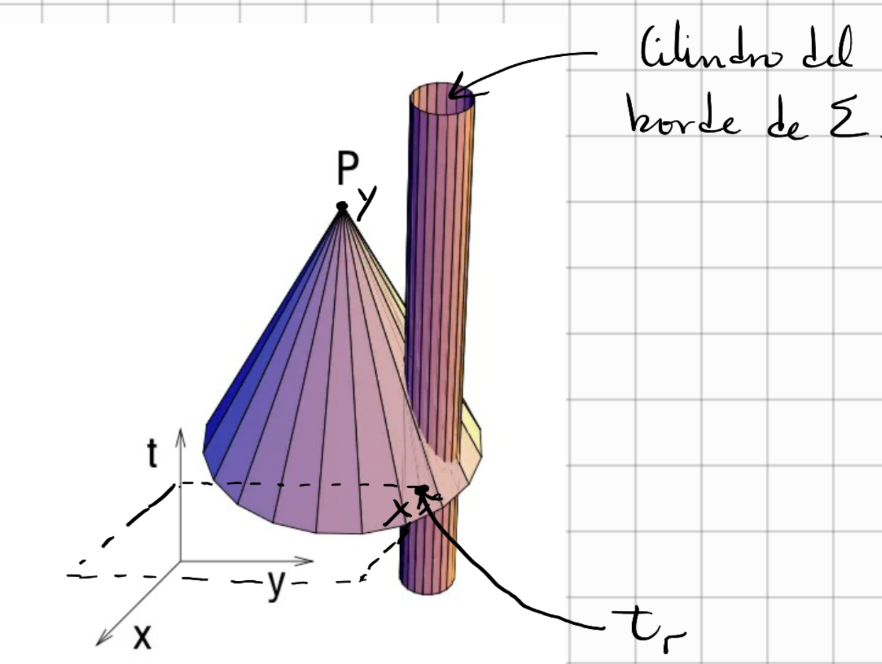
\includegraphics[width=.7\textwidth]{img/imgRG8.2.PNG}
    \label{fig8.2}
    \caption{Geometría para el cono de luz en el pasado de $P$. (Michele Maggiore)}
\end{figure}

La función de Green para el problema homogéneo viene dada por 
\begin{equation}
    G(x-y)=-\dfrac{1}{4\pi} \dfrac{1}{|x-y|}\delta(t_{r+}-t)
\end{equation}

La cantidad $|x-y|$ se puede expandir 
\begin{equation}
    \begin{split}
        |x-y|&=r-\dfrac{x\cdot y}{r} \quad \text{con} \quad r=|x| >> d \\
        \dfrac{1}{|x-y|}&=\dfrac{1}{r}+\dfrac{x\cdot y}{r^3}+\mathcal{O}\left(\dfrac{d^2}{r}\right)
    \end{split}
\end{equation}
donde $d$ es la distancia a la fuente.
\begin{equation}
    T_{\mu\nu}(t_r, y)=T_{\mu\nu}(t-r, y)+\dv{}{t}T_{\mu\nu}(t-r, y)\dfrac{x\cdot y}{r}
\end{equation}
donde esta expansión es válida si $\dot{T}_{\mu\nu} << T_{\mu\nu}$ a primer orden se tiene 
\begin{equation}
    \bar{h}_{\mu\nu}(t, x)=\dfrac{4G}{r}\int_{\Sigma} \mathrm{d^3}y T_{\mu\nu}(t-r, y)+\mathcal{O}\left(\left(\dfrac{d}{r}\right)^2\right)
\end{equation}

Donde las componentes espaciales de $h_{\mu\nu}$ vienen dadas por:
\begin{equation}
    \bar{h}_{ij}(t, x)\approx \dfrac{4G}{r}\int_{\Sigma}\mathrm{d}^3 y T_{ij}(t-r, y)
\end{equation}

Escribiendo $T_{ij}$ en términos de derivadas:
\begin{equation}
    \begin{split}
        T_{ij}&=T_{ik}\delta^k_j+\partial^k T_{ik}y_j-\partial^k T_{ik}y_j \\
        &=T_{ik}\partial^k y_j+\partial^k T_{ik}y_j-\partial^k T_{ik}y_j \\
        &=\partial^k(T_{ik}y_j)-\partial^k T_{ik} y_j
    \end{split}
\end{equation}


\section{Energía Radiada}

\section{Flujo de energía}

\section{Problemas 8}
\begin{enumerate}
    \item \textbf{Parámetros en Inflación}
    
    Derive algunas identidades útiles que involucran los parámetros de desaceleración durante la inflación en tiempo conforme $\tau$.
    \begin{enumerate}[label=(\alph*)]
        \item Demuestra que 
        \begin{equation}
            \dv{}{\tau}\left(\dfrac{1}{aH}\right)=\epsilon-1.
        \end{equation}
        \item Muestre que el factor de Hubble satisface:
        \begin{equation}
            4\pi G(\dot{\phi})^2=\epsilon H^2.
        \end{equation}
        \item Utilizando las definiciones de $\epsilon$ y $\delta$, demuestra que:
        \begin{equation}
            \dv{\epsilon}{t}=-2aH\epsilon(\epsilon+\delta).
        \end{equation}
        \item Expresa los parámetros de desaceleración $\epsilon$ y $\eta$ en términos del potencial $V$ y sus derivadas con respecto a $\phi$. Demuestra que:
        \begin{equation}
            \epsilon=\dfrac{1}{16\pi G}\left(\dfrac{V'}{V}\right)^2
        \end{equation}
        y
        \begin{equation}
            \delta=-\epsilon+\dfrac{1}{8\pi G}\dfrac{V''}{V}
        \end{equation}
        donde las primas denotan derivadas con respecto a $\phi$ para el potencial $V$.
    \end{enumerate}
    \item \textbf{Usando el campo de Higgs como inflación}
    
    En este problema vamos a estudiar si el campo de Higgs puede ser usado para inflación:
    \begin{enumerate}[label=(\alph*)]
        \item Sea el potencial del bosón de Higgs 
        \begin{equation}
            V(\phi)=\lambda(\phi^2-v^2)^2,
        \end{equation}
        donde $v=246$ GeV. Dibuja el potencial e indica las regiones donde podría ocurrir la inflación de lento decaimiento (\textit{slow-roll}). Calcula los parámetros de lento decaimiento $\epsilon_V \equiv \dfrac{1}{2}M^2_{pl}(V'/V)^2$ y $\eta_V \equiv M^2_{pl} (V''/V)$.
        \item Considere la región $0<\phi<v$. Dibuje $\epsilon_V(\phi)$ y $\eta_V(\phi)$ entre $\phi=0$ y $\phi=v$. ¿Existe una región en la cual ambas condiciones de lento decaimiento pueden cumplirse simultáneamente?
        \item Ahora, observe el régimen $\phi >> v$. Demuestra que $\epsilon_V(\phi)$ y $\eta_V(\phi)$ se vuelven independientes de $v$. ¿Para qué valores de campo ocurre la inflación? Determina los valores de campo al final de la inflación $(\phi_E)$ y $N_{\star}\sim 60$ e-dobles antes $(\phi_{\star})$. [Puedes asumir que $\phi_{\star}>>\phi_E$.]
        \item Calcule la amplitud del espectro de potencia de las fluctuaciones escalares en $\phi_{\star}$. Expresa tu respuesta en términos de $N_{\star}$ y la masa del bosón de Higgs $m_H$.
        \item Estima el valor de $m_H$ requerida para igualar la amplitud escalar observada $\Delta^2_s=2\times 10^{-9}$. Compara esto con la masa anunciada del bosón de Higgs, $m_H=125$ GeV.
    \end{enumerate}
    \item \textbf{Ondas Gravitacionales en el vacío}
    
    Para realizar una descripción perturbativa de la gravedad, considere un sistema de coordenadas $(U, x)$ del espacio-tiempo $M$, en el cual la métrica $g$ toma la forma $g_{\mu\nu}(x)\mathrm{d}x^{\mu}\mathrm{d}x^{\nu}$ con:
    \begin{equation}
        g_{\mu\nu}=\eta_{\mu\nu}+h_{\mu\nu},
    \end{equation}
    donde $\eta$ denota la métrica plana de Minkowski. Y limitemos nuestro interés en un sistema de coordenadas donde el régimen de gravedad débil se traduce en $||h_{\mu\nu}||<<1$.
    \begin{enumerate}[label=(\alph*)]
        \item Muestre que: 
        \begin{equation}
            g^{\mu\nu}=\eta^{\mu\nu}-h^{\mu\nu}.
        \end{equation}
        \item Muestre a continuación que los símbolos de Christoffel se leen:
        \begin{equation}
            \Gamma^{\rho}_{\mu\nu}=\dfrac{1}{2}\eta^{\rho\lambda}(\partial_{\mu} h_{\nu\lambda}+\partial_{\nu}h_{\lambda\mu}-\partial_{\lambda}h_{\mu\nu}).
        \end{equation}
        \item Muestre luego que, en el orden en el que estamos trabajando,
        \begin{equation}
            R_{\mu\nu}=\dfrac{1}{2}(\partial_{\sigma}\partial_{\nu}h^{\sigma}_{\mu}+\partial_{\sigma}\partial_{\mu}h^{\sigma}_{\nu}-\partial_{\mu}\partial_{\nu}h-\Box h_{\mu\nu}),
        \end{equation}
        con $h=\eta^{\mu\nu} h_{\mu\nu}=h^{\mu}_{\mu}$ y $\Box$ siendo el D'Alambertiano del espacio plano, $\Box=-\partial^2_t+\partial^2_x+\partial^2_y+\partial^2_z$.
        \item Demuestre que esto se puede convertir en 
        \begin{equation}
            R_{\mu\nu}=\dfrac{1}{2}(\partial_{\mu}\partial^{\lambda}\bar{h}_{\lambda\nu}+\partial_{\nu}\partial^{\lambda}\bar{h}_{\lambda\mu}-\Box h_{\mu\nu}),
        \end{equation}
        con $\bar{h}_{\mu\nu}=h_{\mu\nu}-\dfrac{1}{2}h \eta_{\mu\nu}$, siendo la perturbación inversa de traza.
    \end{enumerate}
    El siguiente paso es lidiar con la libertad de calibre correspondiente a las transformaciones de coordenadas. Suponga que hacemos una buena transformación de coordenadas, tal que 
    \begin{equation}
        x^{\mu} \ \rightarrow \ y^{\mu}(x)=x^{\mu}+\epsilon^{\mu}(x), 
    \end{equation}
    con $|| \epsilon^{\mu} || <<1$ y $|| \partial_{\sigma}\epsilon^{\mu} || <<1$:
    \begin{enumerate}[label=(\alph*), start=5]
        \item Comience con la transformación de la métrica $g$ y demuestre que
        \begin{equation}
            g_{\mu\nu}(y)=\eta_{\mu\nu}+h_{\mu\nu}(y)-\partial_{\mu}\epsilon_{\nu}(y)-\partial_{\nu}\epsilon_{\mu}(y)
        \end{equation}
        \item Ahora podemos volver a la parte (d) y notar que si: 
        \begin{equation}
            \partial^{\mu}\bar{h}_{\mu\nu}=0
        \end{equation}
        hay una notable simplificación en el tensor de Ricci. Fijar el calibre es equivalente a encontrar una transformación de coordenadas específica $\epsilon^{\mu}$. Muestre que para una perturbación dada de la métrica $h$, haciendo una transformación de coordenadas por $\epsilon$ con:
        \begin{equation}
            \Box \epsilon^{\nu}=\partial_{\mu}\bar{h}^{\mu\nu},
        \end{equation}
        se reduce al calibre de Lorenz.
        \item Una vez en el calibre de Lorenz, demuestre que la ecuación linearizada de Einstein se lee:
        \begin{equation}
            \Box \bar{h}_{\mu\nu}=-16\pi G T_{\mu\nu}.
        \end{equation}
        En este punto, podemos especializarnos en el caso de la solución de vacío; es decir, no nos preocupamos por cómo se ha originado una onda gravitacional, sino que nos gustaría saber cómo se propagaría una onda existente.
        \item Verifique que la onda plana 
        \begin{equation}
            \bar{h}_{\mu\nu}(x)=a_{\mu\nu}\exp\left(i(k^{\lambda}x_{\lambda}+\phi)\right),
        \end{equation}
        con $k$ constante, $a$ simétrica constante y fase constante $\phi$, es de hecho una solución a la ecuación linealizada de Einstein al vacío, si $k$ es similar a la luz.
    \end{enumerate}
    \item \textbf{Radiación cuadrupolar en órbitas circulares}
    
    En este problema, consideramos un sistema binario con masas $m_1$ y $m_2$, y asumimos que la coordenada relativa realiza un movimiento circular. Por el momento, asumimos que el movimiento orbital está dado y que descuidamos cualquier retroacción (\textit{backreaction}) en el movimiento debido a la emisión de ondas gravitacionales. Dadas las ecuaciones paramétricas de la órbita en el plano $(x, y)$:
    \begin{equation}
        \begin{split}
            x_0(t)&=R \cos\left(\omega_s t+\dfrac{\pi}{2}\right),\\
            y_0(t)&=R \sin\left(\omega_s t+\dfrac{\pi}{2}\right),\\
            z_0(t)&=0.
        \end{split}
    \end{equation}
    Encuentre:
    \begin{enumerate}[label=(\alph*)]
        \item Las componentes del tensor segundo momento de masa $M^{ij}$.
        \item Encuentre las amplitudes de polarización de las ondas gravitacionales $h_{\times}$, $h_{+}$.
    \end{enumerate}
    \item \textbf{Momento angular de las ondas gravitacionales}
    
    Comenzando por la acción Einstein-Hilbert obtenga para una perturbación de la métrica $g_{\mu\nu}=\eta_{\mu\nu}+h_{\mu\nu}$:
    \begin{equation}
        S_E=-\dfrac{c^3}{64\pi G} \int \mathrm{d}^4 x\left[\partial_{\mu}h_{\alpha\beta}\partial^{\mu}h^{\alpha\beta}-\partial_{\mu}h \partial^{\mu}h+2\partial_{\mu}h^{\mu\nu}\partial_{\nu}h-2\partial_{\mu}h^{\mu\nu}\partial_{\rho}h^{\rho}_{\nu}\right].
    \end{equation}
    Extraiga la expresión siguiente usando los grados de libertad físicos:
    \begin{equation}
        \mathcal{L}=-\dfrac{c^4}{64\pi G}\partial_{\mu}h^{\mathrm{TT}}_{ij}\partial^{\mu}h^{\mathrm{TT}}_{ij}.
    \end{equation}
    Usando el teorema de Noether derive la expresión para el momento angular de una onda gravitacional:
    \begin{equation}
        J^{i}=\dfrac{c^2}{32\pi G}\int \mathrm{d}^3 x\left[-\epsilon^{ikl}h^{\mathrm{TT}}_{ab}x^k \partial^{l}h^{\mathrm{TT}}_{ab}+2\epsilon^{ikl}h^{\mathrm{TT}}_{ak}\dot{h}^{\mathrm{TT}}_{al}\right].
    \end{equation}
\end{enumerate}
\end{document}